
\section{Introduction}

Recent advances in foundational text-to-image (T2I) generative models have demonstrated remarkable capabilities in high-fidelity image synthesis and complex prompt understanding, as discussed in Appendix~\ref{sec:related works}. However, these gains have come at a substantial cost: training such models typically requires massive computational resources, leading to prohibitive financial and environmental expenses. For example, Z-Image~\citep{cai2025zimage} requires approximately 314K H800 GPU hours for pre-training, highlighting the growing scalability challenge of training foundation-scale T2I models.

In this paper, we focus on improving the \textbf{training-time efficiency} of foundational T2I models. We argue that training-time efficiency is jointly determined by three key factors: (1) \textit{model size}, which directly affects the computational cost of each training step; (2) \textit{data information density per training batch}, which determines how much useful supervision the model can extract from each update; and (3) \textit{convergence speed}, which determines the overall number of training iterations, as faster convergence enables the model to achieve strong performance with fewer optimization steps. Therefore, improving training-time efficiency requires not only reducing model scale, but also increasing the learning value of each batch and accelerating convergence throughout training.

Motivated by these factors, we introduce \textbf{Lens}, a foundational T2I model designed for efficient training. First, to reduce the per-step computational cost, we constrain \textit{Lens} to 3.8B parameters. In contrast, recent state-of-the-art open-source models, including Z-Image (6B)~\citep{cai2025zimage}, LongCat-Image (6B)~\citep{team2025longcat}, FLUX.2 (9B)~\citep{flux-2-2025}, Qwen-Image (20B)~\citep{wu2025qwenimage}, and Hunyuan-Image-3.0 (MoE, 80B)~\citep{cao2025hunyuanimage}, operate at scales of 6B parameters or larger. Despite its relatively compact 3.8B-parameter scale, \textit{Lens} achieves performance competitive with, and in several cases surpassing, prior state-of-the-art larger models across multiple benchmarks, as shown in Figure~\ref{fig:benchmark_scatter}, while substantially reducing training cost. For example, compared with Z-Image (6B)~\citep{cai2025zimage}, \textit{Lens} (3.8B) attains competitive or superior results while using only approximately 19.3\% of its training compute.
%, computed as $(192\times312)/(314\times989.5)\approx0.193$. 
Specifically, \textit{Lens} requires 192K A100 GPU hours (312 TFLOPS, BF16), whereas Z-Image requires 314K H800 GPU hours (989.5 TFLOPS, BF16).\footnote{This comparison uses peak BF16 TFLOPS to normalize GPU types. Actual efficiency may differ due to memory bandwidth, MFU, and communication overhead. Re-captioning costs are excluded, as this one-time preprocessing can be reused for future models.} Moreover, due to its smaller model size, \textit{Lens} also enables faster inference under the same number of denoising steps.


Despite its reduced model size, the high training efficiency and strong performance of \textit{Lens} are largely attributed to two additional factors: \textit{data information density per training batch} and \textit{convergence speed}.

\noindent\textbf{Data Information Density per Training Batch.}
Given a training batch consisting of a set of \textit{image-text pairs}, our objective is to maximize the amount of useful visual-semantic supervision contained in each optimization step. To this end, we increase information density from both the text and image perspectives:

\begin{itemize}[leftmargin=*, labelsep=0.3em]
    \item \textbf{Text Information Density.} Conventional short captions provide limited supervision, as they often describe only the most salient object or scene category. In contrast, dense captions encode richer semantic details, including objects, attributes, spatial relationships, actions, and background context, allowing each image-text pair to provide stronger training signals. This effectively increases the text-side information density of the dataset. Accordingly, \textit{Lens} is trained on 800M densely captioned image-text pairs, where each caption is generated by a strong vision-language model, \textit{GPT-4.1}, with an average length of 109 words.
    \item \textbf{Image Information Density.} We increase image-side information density by constructing each training batch from images with multiple resolutions (i.e., $\{512^2, 768^2, 1024^2\}$) and diverse aspect ratios (e.g., $1{:}2$, $9{:}16$, $1{:}1$, and $4{:}3$). This strategy significantly increases image information density within each training batch: multi-resolution training allows the model to learn visual content at different levels of detail, from global scene structure to fine local patterns, while multi-aspect-ratio training exposes it to diverse object arrangements, spatial relationships, and compositional layouts. Moreover, a useful by-product of this strategy is strong \textit{resolution and aspect-ratio generalization} at inference time: the model generalizes well to unseen aspect ratios (e.g., $5{:}4$ and $6{:}7$) and to resolutions up to $1440^2$. This capability removes the need for costly high-resolution training, which further enhances overall training efficiency when high-resolution generation is desired. 
\end{itemize}

\begin{figure*}[t]
  \centering
  \makebox[\textwidth][c]{%
  \begin{minipage}[t]{0.48\textwidth}
    \centering
    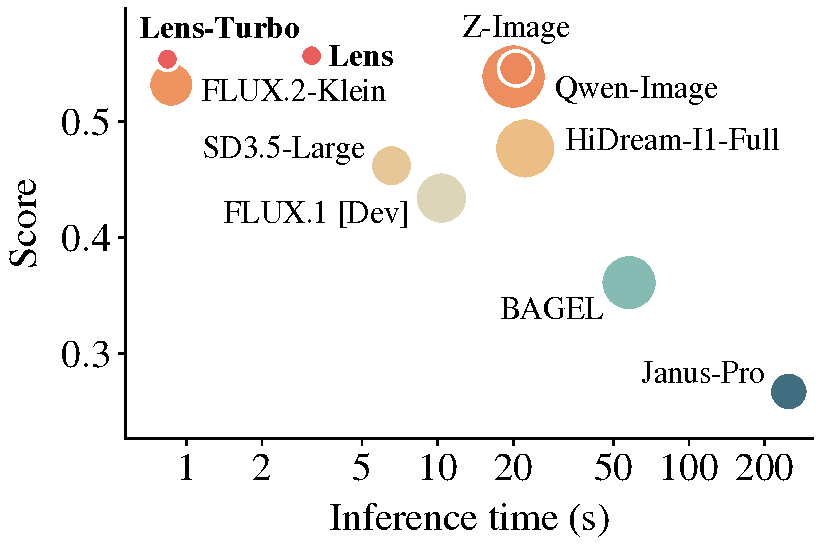
\includegraphics[width=\linewidth]{figures/oneig_scatter.pdf}
    \\[-0.35em]
    \small (a) OneIG
  \end{minipage}
  \hspace{0.01\textwidth}
  \begin{minipage}[t]{0.48\textwidth}
    \centering
    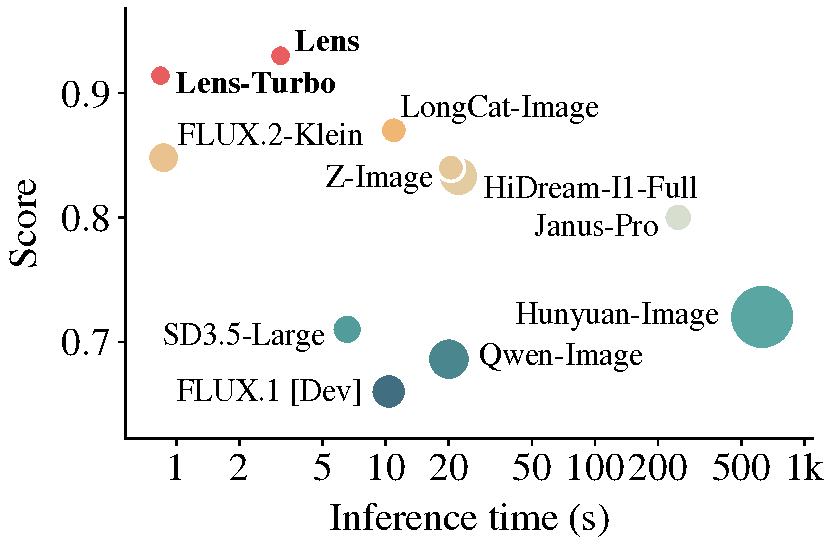
\includegraphics[width=\linewidth]{figures/geneval_scatter.pdf}
    \\[-0.35em]
    \small (b) GenEval
  \end{minipage}%
  }
  %\vspace{-3mm}
  \caption{Comparison of inference time and benchmark performance on OneIG~\citep{chang2025oneigbench} and GenEval~\citep{ghosh2023geneval} across representative T2I models. The $x$-axis denotes inference time on a single NVIDIA H100 GPU, the $y$-axis denotes the benchmark score, and the marker area is proportional to model size.}
  %\vspace{-3mm}
  \label{fig:benchmark_scatter}
\end{figure*}

\noindent\textbf{Convergence Speed.} \textit{Lens} further enhances training efficiency by accelerating optimization convergence. We explore several architectural design choices that allow the model to learn more effectively and reach strong performance with fewer training iterations. These studies include:

\begin{itemize}[leftmargin=*, labelsep=0.3em]
\item \textbf{VAE Variants.} We systematically study different VAE variants, including conventional VAEs used in FLUX.1~\citep{flux2024} and SD3~\citep{esser2024scaling}, as well as semantic VAEs adopted in FLUX.2~\citep{flux-2-2025} and VTP~\citep{vtp}. Instead of relying on proxy metrics such as rFID or class-conditional ImageNet generation, we directly evaluate each VAE within the T2I pipeline using a 130M subset of our training data. 

\item \textbf{Language Encoder Variants.} The language encoder provides text-conditioning features for diffusion modeling. We find that stronger language encoders not only accelerate optimization convergence but also improve multilingual generalization. Specifically, although the model is trained only on English image-text pairs, a strong language encoder enables robust inference-time generalization to other languages, such as Chinese and French. This multilingual generalization substantially reduces data requirements and training costs in scenarios where the model needs to handle multilingual inputs. Based on careful ablation studies, we adopt GPT-OSS~\citep{openai2025gptoss120bgptoss20bmodel} as the language encoder.
\end{itemize}


After efficient pre-training, \textit{Lens} generates diverse images, but their aesthetic quality may vary and some outputs may contain artifacts. We apply reinforcement learning (RL) as a post-training step to suppress artifacts, improve visual composition, and enforce consistency with real-world physical rules. A key finding is that RL data must be sufficiently diverse and cover the original training distribution to avoid performance degradation on certain input types. To this end, we construct the \textit{Lens-RL-8K} prompt set with taxonomy-driven coverage of diverse generation scenarios. Experiments show that post-training on \textit{Lens-RL-8K} significantly improves generation performance across a broad range of scenarios.



Additionally, following modern T2I systems, we equip \textit{Lens} with a \textit{reasoner} module that can be instantiated with different LLMs. The reasoner converts ambiguous or underspecified user requests into detailed prompts aligned with the training-caption distribution. It takes the user request and a system prompt as input, where the system prompt specifies guidelines for constructing suitable T2I prompts. We further introduce a \textit{training-free system prompt search strategy} to optimize these guidelines, enabling the reasoner to generate prompts that better align with the T2I model. Note that reasoner-based prompt rewriting is now a standard practice in modern T2I systems; to ensure a fair comparison, we report results both with and without the reasoner in our experiments.

Overall, in this paper we systematically investigate a set of training efficiency factors that are often overlooked in practice, including data captioning strategies, VAE selection criteria, language encoder choices, and training-data composition for RL-based post-training. For each factor, we provide controlled ablation studies with quantitative analysis, yielding actionable insights for building T2I foundation models. Importantly, these strategies are complementary to conventional training acceleration approaches, such as architectural innovations and distributed-system optimization. Guided by these findings, \textit{Lens} achieves performance competitive with larger state-of-the-art models at substantially lower training cost. Its compact model size also enables faster inference: by default, \textit{Lens} generates a $1024^2$ image in \textbf{3.15} seconds on a single NVIDIA H100 GPU using 20 denoising steps, while \textit{Lens-Turbo}, a 4-step distilled variant, further reduces the generation time to \textbf{0.84} seconds.
